\documentclass[12pt]{article}
\usepackage{graphicx}
\graphicspath{ {images/} }
\usepackage[spanish]{babel}
\usepackage[utf8]{inputenc}
\usepackage[backend=biber]{biblatex}
\usepackage[T1]{fontenc}
\usepackage{lmodern}

\begin{document}

\thispagestyle{empty}
\begin{center}
\begin{figure}[h]
\centering

\includegraphics[width=.6\textwidth]{logo.jpg}\\
\end{figure}

\vspace{1cm}
\Large \sc  Instituto Tecnológico y de Estudios Superiores de Monterrey
\\

\vspace{2.5cm}
\Large \bf
\emph{Actividad 1. Conceptos básicos de ciencia de datos}

\vspace{2.5cm}
\Large \bf Aarón Hernández Jiménez\\
\vspace{0.3cm}
\Large \bf A01642529\\
\vspace{3.5cm}
\normalsize \sc \rightline{Ciencia y analítica de datos}
\vspace{0.3cm}
\normalsize \sc \rightline{22 de noviembre de 2026}
\end{center}

\newpage

\section{Relación entre los conceptos}
La siguiente figura muestra la relación entre los términos: ciencia de datos (\emph{data science}), aprendizaje automático (\emph{machine learning}) y minería de datos (\emph{data mining}). \\

\begin{figure}[!h]
\centering{
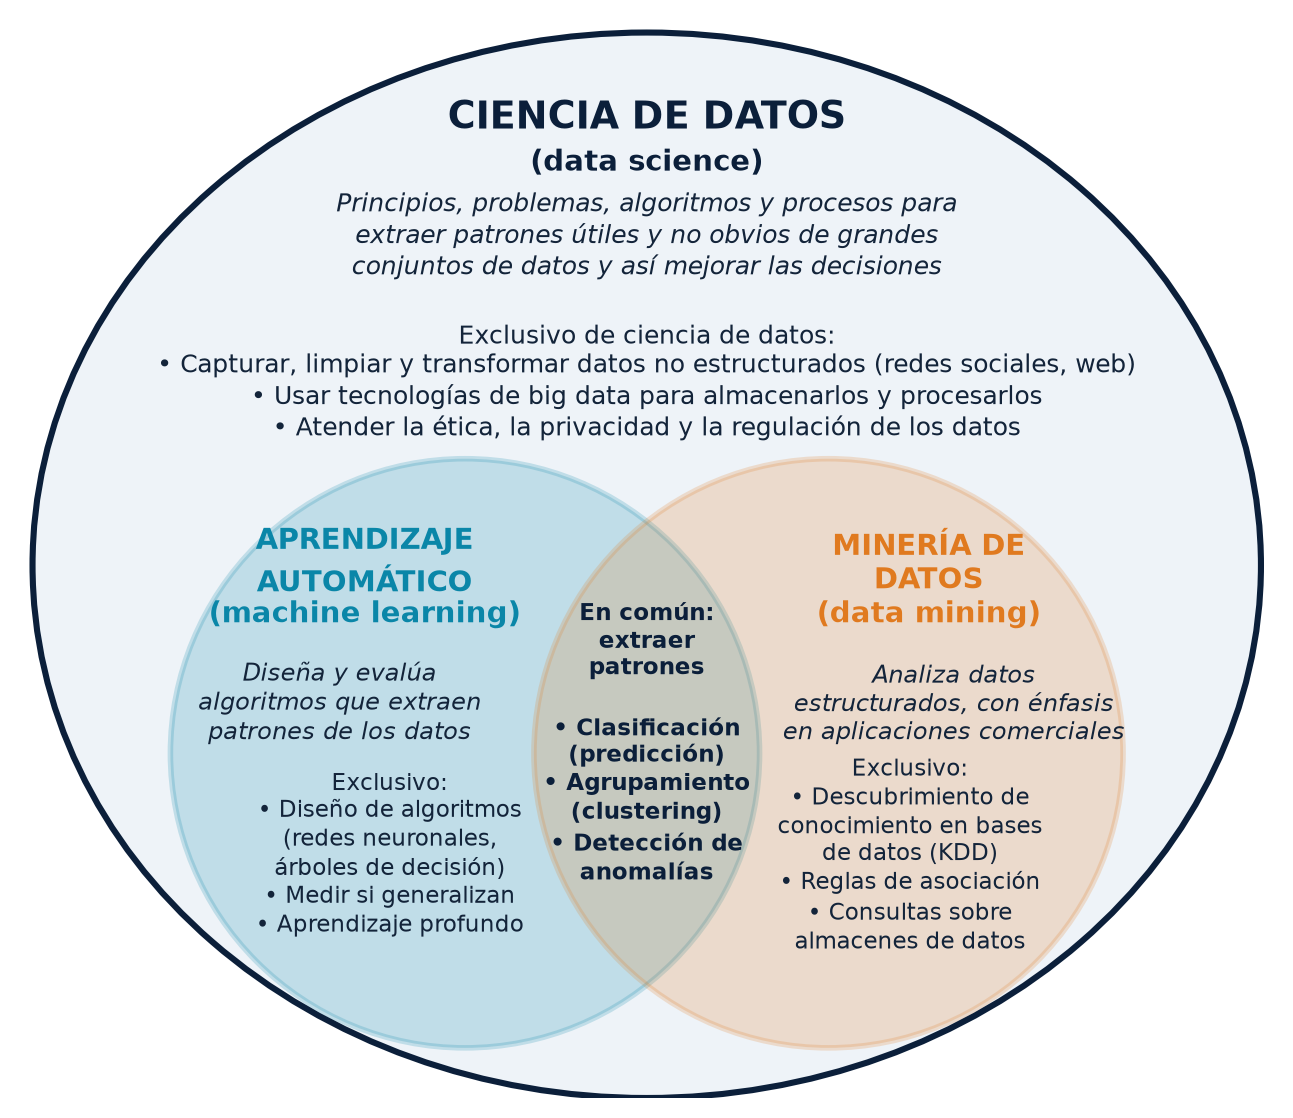
\includegraphics[width=1\textwidth]{diagrama.png}\\
\caption{Relación entre ciencia de datos, aprendizaje automático y minería de datos. Elaboración propia con base en \cite{1} y \cite{2}.}}
\end{figure}

Los tres términos comparten el objetivo de mejorar las decisiones mediante el análisis de datos, pero la ciencia de datos es la más amplia: incluye al aprendizaje automático y a la minería de datos, y además atiende retos propios como los datos no estructurados, el \emph{big data} y la ética \cite{1}, \cite{2}.


\newpage
\section{Elementos del aprendizaje estadístico}

\begin{itemize}
    \item \textsc{Regla de Bayes}: Laplace retomó las ideas de Thomas Bayes y Richard Price y formuló la primera versión de esta regla, que permite actualizar la probabilidad de una hipótesis cuando aparece nueva evidencia: $P(H\mid E)=P(E\mid H)\,P(H)/P(E)$ \cite{1}. \emph{Ejemplo:} un filtro de correo estima la probabilidad de que un mensaje sea \emph{spam} sabiendo que contiene la frase ``gana dinero fácil'', a partir de qué tan seguido aparece esa frase en correos \emph{spam} y en correos normales \cite{3}.

    \item \textsc{Método de mínimos cuadrados}: Gauss lo desarrolló al buscar el planeta enano Ceres; encuentra el modelo que mejor se ajusta a los datos minimizando la suma de los cuadrados de las diferencias entre cada dato y el modelo. Es la base de la regresión lineal y de la regresión logística \cite{1}, \cite{3}. \emph{Ejemplo:} estimar el precio de un diamante a partir de su peso en quilates con una recta de regresión, como en la actividad de regresión lineal del curso.
\end{itemize}

\section{Elementos del aprendizaje automático}

\begin{itemize}
    \item \textsc{Árboles de decisión}: en 1966 Hunt, Marin y Stone propusieron el \emph{concept-learning system}, origen de la familia de algoritmos que construyen árboles de decisión de arriba hacia abajo \cite{1}. El árbol divide los datos, paso a paso, según el atributo que mejor separa las clases y produce reglas del tipo ``si\ldots{} entonces\ldots'' fáciles de explicar \cite{4}. \emph{Ejemplo:} decidir si un cliente aceptará un préstamo personal según su ingreso, su escolaridad y si tiene cuenta de inversión.

    \item \textsc{Agrupamiento \emph{k-means}}: a mediados de los sesenta varios investigadores publicaron versiones de este algoritmo, hoy el estándar para segmentar clientes \cite{1}. Asigna cada registro al más cercano de $k$ centros y recalcula los centros hasta que los grupos ya no cambian \cite{2}. \emph{Ejemplo:} una tienda en línea agrupa a sus clientes por frecuencia y monto de compra para diseñar una promoción distinta para cada segmento.
\end{itemize}

\newpage
\section*{Declaración de uso de IA}
Anthropic. (2026). Claude (Opus 5.5) [Modelo de lenguaje grande], utilizado para localizar los elementos en la lectura, apoyar la redacción, generar el código del diagrama y compilar el documento \cite{5}. El contenido fue revisado por el autor.

\begin{thebibliography}{a}

\bibitem{1}
John D. Kelleher and Brendan Tierney, \emph{Data Science}, The MIT Press Essential Knowledge Series. Cambridge, MA: The MIT Press, 2018, cap. 1, pp. 1--24.

\bibitem{2}
Jiawei Han, Micheline Kamber and Jian Pei, \emph{Data Mining: Concepts and Techniques}, 3rd ed. Waltham, MA: Morgan Kaufmann, 2011.

\bibitem{3}
Gareth James, Daniela Witten, Trevor Hastie and Robert Tibshirani, \emph{An Introduction to Statistical Learning with Applications in R}, 2nd ed. New York: Springer, 2021.

\bibitem{4}
Tom M. Mitchell, \emph{Machine Learning}. New York: McGraw-Hill, 1997.

\bibitem{5}
Anthropic, Claude (Opus 5.5) [Modelo de lenguaje grande], 2026. \\ \url{https://claude.ai} (visitado 22-11-2026)

\end{thebibliography}

\end{document}
